\documentclass{beamer}

% \usepackage{beamerthemesplit} // Activate for custom appearance

\title{Applied Regression}
\author{Frank Wood}
%\date{\today}

\newcommand{\comment}[1]{}
\newcommand{\ponedec}{\mathcal{P}^\downarrow_1}
\newcommand{\pone}{\mathcal{P}_1}
\newcommand{\rank}[1]{\mathrm{RANK}\left[#1\right]}
\newcommand{\E}[1]{\mathrm{E}\left[#1\right]}
\newcommand{\py}{\mathcal{PY}}
\newcommand{\iid}{iid.}
\newcommand{\drawiid}{\stackrel{\text{iid}}{\sim}}
\newcommand{\vect}[1]{\mathbf{#1}}
\newcommand{\indicator}[1]{\text{I}\left[ #1 \right]}
\newcommand{\pdcoag}{PD(d_1,0)-\text{COAG}}
\newcommand{\todo}{\textbf{*TODO*}}
\newcommand{\igram}{\text{$\infty$-gram}}
\newcommand{\Prob}{\text{P}}

\def\mm{sequence memoizer }
\def\MM{SM }

\def\pibf{{\boldsymbol{\pi}}}
\def\kapbf{\boldsymbol{\kappa}}
\def\taubf{\boldsymbol{\tau}}
\def\thebf{\boldsymbol{\theta}}
\def\rhobf{\boldsymbol{\rho}}
\def\phibf{\boldsymbol{\phi}}
\def\pbf{\mathbf{p}}
\def\qbf{\mathbf{q}}
\def\sbf{\mathbf{s}}
\def\tbf{\mathbf{t}}
\def\ybf{\mathbf{y}}
\def\wbf{\mathbf{w}}
\def\xbf{\mathbf{x}}
\def\rbf{\mathbf{r}}
\def\tbf{\mathbf{t}}
\def\kbf{\mathbf{k}}
\def\Xbf{\mathbf{X}}
\def\0bf{\mathbf{0}}
\def\Ibf{\mathbf{I}}
\def\phibf{\mathbf{\phi}}
\def\Phibf{\mathbf{\Phi}}
\def\disteq{{\stackrel{D}{=}}}
\def\EE{{\mathbb{E}}}

\def\phiv{\varphi}
\def\phivbf{\boldsymbol{\varphi}}

\def\Ocal{\mathcal{O}}

\DeclareMathOperator*{\Bet}{Beta} \DeclareMathOperator{\coag}{COAG}
\DeclareMathOperator{\frag}{FRAG} \DeclareMathOperator*{\rnk}{RANK}
\DeclareMathOperator*{\gem}{GEM} \DeclareMathOperator*{\pd}{PD}
\DeclareMathOperator*{\gd}{GDir} \DeclareMathOperator*{\Dir}{Dir}
\DeclareMathOperator*{\Ave}{\mathbb{E}}
\DeclareMathOperator*{\Var}{Var}

\begin{document}

\frame{\titlepage}

%\section[Outline]{}
%\frame{\tableofcontents}
%
%\section{Introduction}
%\subsection{Overview of Topics}
%
%\section{Bayesian Analysis}
%\subsection{Single Parameter Model}


\frame[t] {
 \frametitle{Extra Sums of Squares}
 \begin{itemize}
 \item A topic unique to multiple regression
 \item An extra sum of squares measures the marginal decrease in the
 error sum of squares when on or several predictor variables are
 added to the regression model, given that other variables are
 already in the model.
 \item Equivalently-one can view an extra sum of squares as
 measuring the marginal increase in the regression sum of squares
 \end{itemize}
}

\frame[t] {
 \frametitle{Example}
 \begin{itemize}
 \item Multiple regression\\
 -- Output: Body fat percentage
 -- Input: \\
    1. triceps skin fold thickness($X_1$)\\
    2. thigh circumference ($X_2$)\\
    3. midarm circumference ($X_3$)
 \item Aim\\
 --Replace cumbersome immersion procedure with model.
 \item Goal\\
 -- Determine which predictor vafriables provide a good model.
\end{itemize}

}

\frame[t] {
 \frametitle{The Data}
 \begin{figure}[h!]
   \centering
     \caption{}
     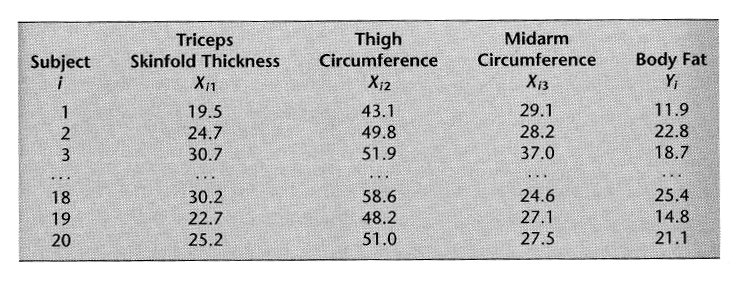
\includegraphics[scale=.4]{4.png}
 \end{figure}
}

\frame[t] {
 \frametitle{Regression of Y on $X_1$}
 \begin{figure}[h!]
   \centering
     \caption{}
     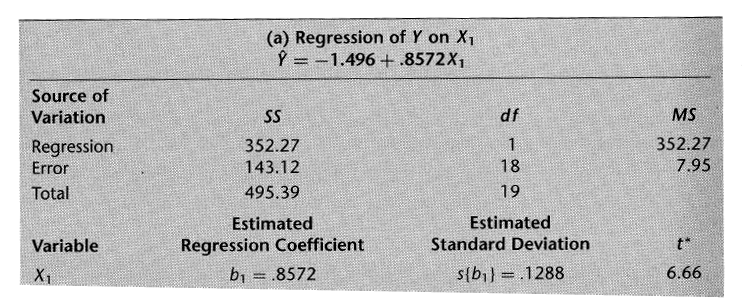
\includegraphics[scale=.4]{5.png}
 \end{figure}
}


\frame[t] {
 \frametitle{Regression of Y on $X_2$}
 \begin{figure}[h!]
   \centering
     \caption{}
     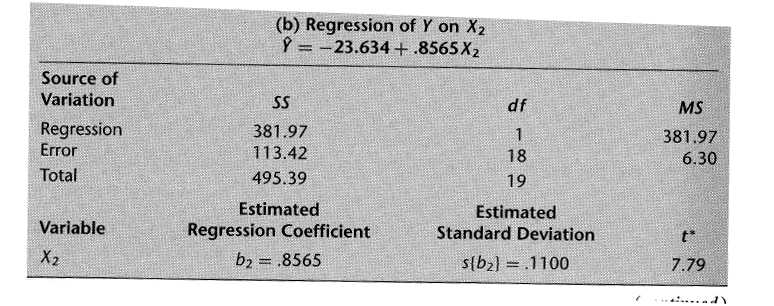
\includegraphics[scale=.4]{6.png}
 \end{figure}
}

\frame[t] {
 \frametitle{Regression of Y on $X_1$ and $X_2$}
 \begin{figure}[h!]
   \centering
     \caption{}
     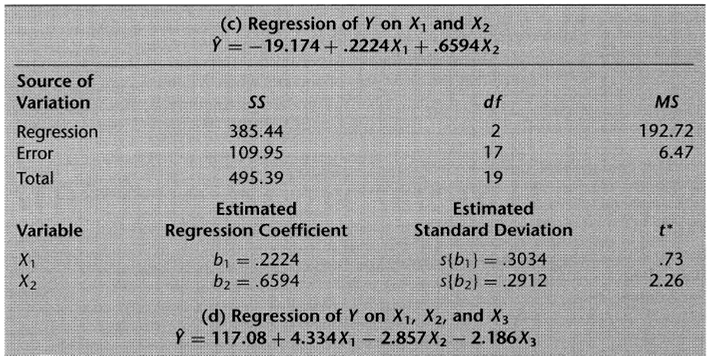
\includegraphics[scale=.4]{7.png}
 \end{figure}
}


\frame[t] {
 \frametitle{Regression of Y on $X_1$ and $X_2$ cont.}
 \begin{figure}[h!]
   \centering
     \caption{}
     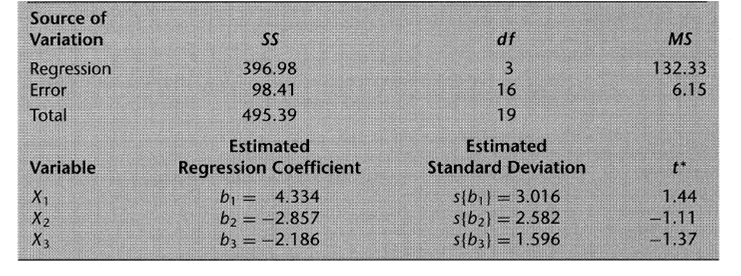
\includegraphics[scale=.4]{8.png}
 \end{figure}
}

\frame[t] {
 \frametitle{Notation}
 \begin{itemize}
 \item SSR $X_1$ only denoted by -SSR($X_1$)=352.27
 \item SSE $X_1$ only denoted by -SSE($X_1$)=143.12
\item Accordingly, \\
--SSR($X_1,X_2$)=385.44\\
--SSE($X_1,X_2$)=109.95
 \end{itemize}
}

\frame[t] {
 \frametitle{More Powerful Model, Smaller SSE}
 \begin{itemize}
 \item When $X_1$ and $X_2$ are in the model, SSE($X_1,X_2$)=109.95
 is smaller than when the model contains only $X_1$
 \item The difference is called an extra sum of squares and will be
 denoted by\\
 --$SSR(X_2|X_1)=SSE(X_1)-SSE(X_1,X_2)=33.17$
 \item The extra sum of squares $SSR(X_2|X_1)$ measure the marginal
 effect of adding $X_2$ to the regression model when $X_1$ is
 already in the model
 \end{itemize}
}

\frame[t] {
 \frametitle{SSR increase <-> SSE decrease}
 The extra sum of squares $SSR(X_1|X_2)$ can equivalently be viewed
 as the marginal increase in the regression sum of squares.\\
 --$SSR(X_2|X_1)=SSR(X_1,X_2)-SSR(X_1)$\\
 --$=385.44-352.27=33.17$
}

\frame[t] {
 \frametitle{Why does this relationship exist?}
 \begin{itemize}
 \item Remember $SSTO=SSR+SSE$
 \item SSTO measures only the variability of the Y's and does not
 depend on the regression model fitted.
 \item Any increase in SSR must be accompanied by a corresponding
 decrease in the SSE.
 \end{itemize}

}

\frame[t] {
 \frametitle{Example relations}
 $SSR(X_3|X_1,X_2)=SSE(X_1,X_2)-SSE(X_1,X_2,X_3)=11.54$\\
 or $SSR(X_3|X_1,X_2)=SSR(X_1,X_2,X_3)-SSR(X_1,X_2)=11.54$\\
 or with multiple variables included at time\\
 --$SSR(X_2,X_3|X_1)=SSE(X_1)-SSE(X_1,X_2,X_3)=44.71$\\
 --or $SSR(X_2,X_3|X_1)=SSR(X_1,X_2,X_3)-SSR(X_1)=44.71$
}

\frame[t]{
 \frametitle{Extra sums of squares}
 An extra sum of squares always involves the difference between the
 error sum of squares for the regression model containing the X
 variables in the model already the error sum of squares for the
 regression model containing both the original X variables and the
 new X variables.
}

\frame[t] {
 \frametitle{Definitions}
 \begin{itemize}
 \item Definition \\
 --$SSR(X_1|X_2)=SSE(X_2)-SSE(X_1,X_2)$
 \item Equivalently \\
 --$SSR(X_1|X_2)=SSR(X_1,X_2)-SSR(X_2)$
 \item We can switch the order of $X_1$ and $X_2$ in these
 expressions
 \item We can easily generalize these definitions for more than two
 variables\\
 --$SSR(X_3|X_1,X_2)=SSE(X_1,X_2)-SSE(X_1,X_2,X_3)$\\
 --$SSR(X_3|X_1,X_2)=SSR(X_1,X_2,X_3)-SSR(X_1,X_2)$
 \end{itemize}

}

\frame[t] {
 \frametitle{N! different partitions}
\begin{figure}[h!]
   \centering
     \caption{}
     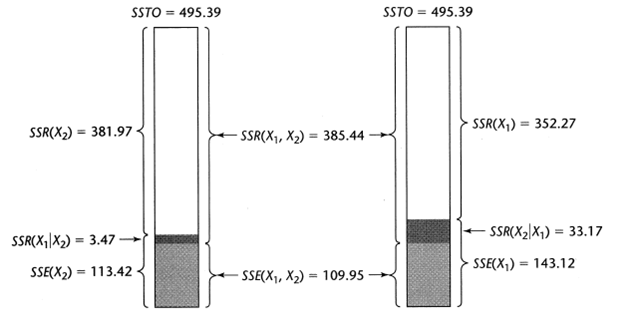
\includegraphics[scale=.4]{16.png}
 \end{figure}

}

\frame[t] {
 \frametitle{ANOVA Table}
 Various software packages can provide extra sums of squares for
 regression analysis. These are usually provided in the order in
 which the input variables are provided to the system, for instance
 \begin{figure}[h!]
   \centering
     \caption{}
     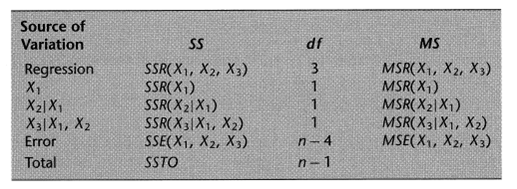
\includegraphics[scale=.4]{17.png}
 \end{figure}
}

\frame[t] {
 \frametitle{Why? Who cares? }
 Extra sums of squares are of interest because they occur in a
 variety of tests about regression coefficients where the question
 of concern is whether certain X variables can be dropped from the
 regression model.
}

\frame[t] {
 \frametitle{Test whether a single $\beta_k=0$}
 \begin{itemize}
 \item Does $X_k$ provide statistically significant improvement to
 the regression model fit?
 \item We can use the general linear test approach
 \item Example\\
 --First order model with three predictor variables\\
 $Y_i=\beta_)+\beta_1 X_{i1}+\beta_2 X_{i2}+\beta_3
 X_{i3}+\epsilon_i$\\
 --We want to answer the following hypotheses test\\
 \begin{center}
$H_0: \beta_3=0$\\
$H_1: \beta_3 \neq 0$
 \end{center}
 \end{itemize}

}

\frame[t]{
 \frametitle{Test whether a single $\beta_k=0$}
 \begin{itemize}
 \item For the full model we have $SSE(F)=SSE(X_1,X_2,X_3)$
 \item The reduced model is $Y_i=\beta_)+\beta_1 X_{i1}+\beta_2 X_{i2}+\epsilon_i$
 \item And for this model we have $SSE(R)=SSE(X_1,X_2)$
 \item Where there are $df_r=n-3$ degrees of freedom associated with
 the reduced model
 \end{itemize}

}


\frame[t]{
 \frametitle{Test whether a single $\beta_k=0$}
 The general linear test statistics is \\
 \begin{center}
 $F^*=\frac{SSE(R)-SSE(F)}{df_R-df_F}/\frac{SSE(F)}{df_F}$
  \end{center}
 which becomes
 \begin{center}
 $F^*=\frac{SSE(X_1,X_2)-SSE(X_1,X_2,X_3)}{(n-3)-(n-4)}/\frac{SSE(X_1,X_2,X_3)}{n-4}$

  \end{center}
 but $SSE(X_1,X_2)-SSE(X_1,X_2,X_3)=SSR(X_3|X_1,X_2)$

 }

\frame[t] {
 \frametitle{Test whether a single $\beta_k=0$}
The general linear test statistics is \\
 \begin{center}
 $F^*=\frac{SSR(X_3|X_1,X_2)}{1}/\frac{SSE(X_1,X_2,X_3)}{n-4}=\frac{MSR(X_3|X_1,X_2)}{MSE(X_1,X_2,X_3)}$
  \end{center}
 Extra sum of squares has one associated degree of freedom.
}

\frame[t] {

 \frametitle{Example}
 Body fat: Can $X_3$ (midarm circumference) be dropped from the
 model?
 \begin{figure}[h!]
   \centering
     \caption{}
     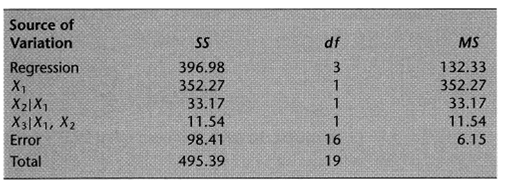
\includegraphics[scale=.4]{23.png}
 \end{figure}
$F^*=\frac{SSR(X_3|X_1,X_2)}{1}/\frac{SSE(X_1,X_2,X_3)}{n-4}=1.88$

}

\frame[t] {
 \frametitle{Example Cont.}
 \begin{itemize}
 \item For $\alpha=.01$ we require $F(.99;1,16)=8.53$
 \item We observe $F^*=1.88$
 \item We conclude $H_0: \beta_3=0$
 \end{itemize}
}

\frame[t] {
 \frametitle{Test whether $\beta_k=0$}
 Another example \\
 $H_0: \beta_2=\beta_3=0$\\
 $H_1:$ not both $\beta_2$ and $\beta_3$ are zero\\
 The general linear test can be used again
\begin{center}
 $F^*=\frac{SSE(X_1)-SSE(X_1,X_2,X_3)}{(n-2)-(n-4)}/\frac{SSE(X_1,X_2,X_3)}{n-4}$

  \end{center}
  But $SSE(X_1)-SSE(X_1,X_2,X_3)=SSR(X_2,X_3|X_1)$\\
  so the expression can be simplified.


}

\frame[t] {
 \frametitle{Tests concerning regression coefficients}
 Summary:\\
 -- General linear test can be used to determine whether or not
 a predictor variable( or sets of variables) should be included in
 the model\\
 -- The ANOVA SSE's can be used to compute $F^*$ test statistics\\
 -- Some more general tests require fitting the model more than once
 unlike the examples given.
}

\frame[t] {
 \frametitle{Standardized Multiple Regression}
 \begin{itemize}
 \item Numerical precision errors can occur when \\
 - $(X'X)^{-1}$ is poorly conditioned near singular : colinearity\\
 - And when the predictor variables have substantially different
 magnitudes
 \item Solution\\
 -- Regularization\\
 -- Standardized multiple regression
 \item First, transformed variables
 \end{itemize}
}

\frame[t] {
 \frametitle{Correlation Transformation}
 Makes all entries in $X'X$ matrix for the transformed variables
 fall between -1 and 1 inclusive\\
 Another motivation\\
 -- Lack of comparability of regression coefficients \\
 $\hat{Y}=200+20000X_1+.2X_2$\\
 $Y$ in dollars, $X_1$ in thousand dollars, $X_2$ in cents\\
 -- Which is most important predictor?
  }

\frame[t] {
 \frametitle{Correlation Transformation}
 1. Centering
 \begin{center}
 $\frac{Y_i-\bar{Y}}{s_y}$\\
 $\frac{X_{ik}-\bar{X}}{s_k}, k-1,...,p-1$
 \end{center}
 2. Scaling
\begin{center}
 $s_y=\sqrt{\frac{\sum(Y_i-\bar{Y})^2}{n-1}}$\\
 $s_k=\sqrt{\frac{\sum(X_{ik}-\bar{X_k})^2}{n-1}}, k-1,...,p-1$
 \end{center}
}

\frame[t] {
 \frametitle{Correlation Transformation}
 Transformed variables\\
 $Y_i^*=\frac{1}{\sqrt{n-1}}(\frac{Y_i-\bar{Y}}{s_y})$\\
 $X_{ik}^*=\frac{1}{\sqrt{n-1}}(\frac{X_{ik}-\bar{X_k}}{s_k}),k=1,...,p-1$
}

\frame[t] {
 \frametitle{Standardized Regression Model}
  Define the matrix consisting of the transformed X variables\\
  \[X= \begin{pmatrix}
 X_{11} &...& X_{1,p-1}\\
 X_{21} &...& X_{2,p-1}\\
 ...\\
 X_{n1} & ... & X_{n,p-1}
  \end{pmatrix}\]\\
 And define $X'X=r_{xx}$

}

\frame[t] {
 \frametitle{Correlation matrix of the X variables}
 Can show that \\
 \[r_{xx}=\begin{pmatrix}
 1 &r_{12}&...&r_{1,p-1}\\
 r_{21} & 1 &...& r_{2,p-1}\\
 ...\\
 r_{p-1,1} & r_{p-1,2}&...&1
 \end{pmatrix}\]
 where each entry is just the coefficient of correlation between
 $X_i$ and $X_j$\\
 \begin{align*}
 \sum x^*_{i1}x^*_{i2}&=\sum
 (\frac{X_{i1}-\bar{X_1}}{\sqrt{n-1}s_1})(\frac{X_{i2}-\bar{X_2}}{\sqrt{n-1}s_2})\\
                            &=\frac{1}{n-1}\frac{\sum
                            (X_{i1}-\bar{X_1})(X_{i2}-\bar{X_2})}{s_1s_2}\\
                            &=\frac{\sum(X_{i1}-\bar{X_1})(X_{i2}-\bar{X_2})}{[\sum(X_{i1}-\bar{X_1})^2\sum(X_{i2}-\bar{X_2})^2]^{1/2}}
\end{align*} }

\frame[t] {
 \frametitle{Standardized Regression Model}
 \begin{itemize}
 \item If we define in a similar way $X'Y=r_{yx}$, where $r_{yx}$ is the
 coefficient of simple correlations between the response variable Y
 and $X_j$\\
 \item Then we can set up a standard linear regression problem\\
 \begin{center}
 $r_{xx}b=r_{yx}$
 \end{center}
\end{itemize}
}

\frame[t] {
 \frametitle{Standardized Regression Model}
 The solution\\
 \[\textbf{b}= \begin{pmatrix}
 b_1^*\\
 b_2^*\\
 .\\
 .\\
 .\\
  b_{p-1}^*\\
 \end{pmatrix}\]\\
 can be related to the solution to the untransformed regression
 problem through the relationship\\
 \begin{center}
 $b_k=(\frac{s_y}{s_k})b_k^*, k=1,...,p-1$\\
 $b_0=\bar{Y}-b_1 \bar{X_1}-...-b_{p-1}\bar{X}_{p-1}$
 \end{center}
}

\frame[t] {
 \frametitle{Multi-colinearity}
 \begin{itemize}
 \item Brief summary
 \item $(X'X)^{-1}$ must be full rank to compute the regression
 solution\\
 --$rank(AB)<=min(rank(A),rank(B))$
 \item Multi-colinearity means that rows of X are linearly dependent
 \item Regression solution is degenerate
 \item High degrees of colinearity produce numerical instability
 \item Very important to consider in real world applications
 \end{itemize}

}












\end{document}
